\documentclass[8pt,aspectratio=169]{beamer}
\usetheme{Boadilla}


\usepackage[utf8]{inputenc}
\usepackage{dsfont}

\usepackage{hyperref}
\usepackage{graphicx}
\usepackage{caption}
\usepackage{subcaption}
%\usepackage{amsmath,amssymb,physics}

\usepackage{amsmath, amssymb, amscd, amsfonts, mathtools, physics, hyperref, color}

\usepackage{tikz}

% Set beamer color info
\definecolor{BIBlue}{RGB}{0,50,150}
\setbeamercolor{title}{fg=black}
\setbeamercolor{frametitle}{fg=black}
\setbeamercolor{structure}{fg=BIBlue}


%Stolen from https://tex.stackexchange.com/questions/388344/beamer-adding-some-text-in-subsection-title-page
\setbeamertemplate{section page}
{
    \begingroup
    \begin{beamercolorbox}[sep=10pt,center,rounded=true,shadow=true]{section title}
        \usebeamerfont{section title}\insertsection\par
    \end{beamercolorbox}
    \endgroup
}

\title{Beyond Class Balance:}
\subtitle{
    Dataset Diversity and Model Performance in Deep-Learning Classification Tasks
    \\
    Award Title: ENRICHing NIH Imaging Datasets to Prepare them for Machine Learning
    }
\institute{
    Beth Israel Deaconess Medical Center\\
}

\author{
    Josiah Couch, Ph.D.\\
    PIs: Rima Arnaout, M.D. and Ramy Arnaout, M.D., D.Phil.
    }
%\institute{Beth Israel Deaconess Medical Center}
\date{27 March 2024}



\begin{document}

\begin{frame}
\titlepage
\end{frame}

%\begin{frame}
%\frametitle{Outline}
%\tableofcontents[]
%\end{frame}

\section{Introduction}
%\begin{frame}
%\sectionpage
%\end{frame}


\subsection{Motivation}
\begin{frame}
\frametitle{Motivation}

\onslide<1->{
\begin{minipage}[t]{0.45\linewidth}

    \begin{itemize}
        \item \onslide<2->{We want to understand dataset quality}
        \begin{itemize}
            \item \onslide<3->{high quality dataset $\rightarrow$ high performance model}
        \end{itemize}
        \item \onslide<4->{In particular, what indicators diagnose a dataset as high quality?}
        \begin{itemize}
            \item \onslide<5->{Class balance}
            \item \onslide<6->{Dataset size}
            \item \onslide<7->{Other things?}
        \end{itemize}
        \item \onslide<8->{There must be more to quality than class balance and size}
        \item \onslide<9->{Just look at these two datasets $\rightarrow$}
        \begin{itemize}
            \item \onslide<10->{Same class balance}
            \item \onslide<11->{Same number of images}
            \item \onslide<12->{But dataset 1 clearly has higher diversity}
            \item \onslide<13->{And thus perhaps a higher quality?}
        \end{itemize}
        \item \onslide<14->{Our starting hypothesis is that diversity contributes to quality independently of class balance (and of dataset size)}
    \end{itemize}

\end{minipage}}
%
\hfill
%
\begin{minipage}[t]{0.45\linewidth}
\onslide<9->{
    \begin{figure}
        \begin{center}
        
        \begin{subfigure}[b]{0.2\textwidth}
             \centering
             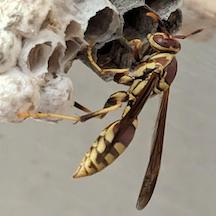
\includegraphics[width=\textwidth]{slide_img/wasp1.jpeg}
         \end{subfigure}   
         %
        \begin{subfigure}[b]{0.2\textwidth}
             \centering
             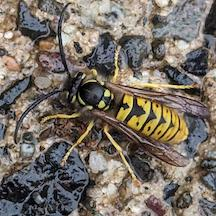
\includegraphics[width=\textwidth]{slide_img/wasp2.jpeg}
         \end{subfigure}
         %
        \begin{subfigure}[b]{0.2\textwidth}
             \centering
             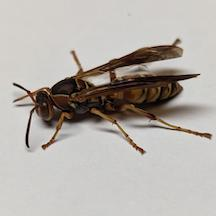
\includegraphics[width=\textwidth]{slide_img/wasp3.jpeg}
         \end{subfigure} 
         %
        \begin{subfigure}[b]{0.2\textwidth}
             \centering
             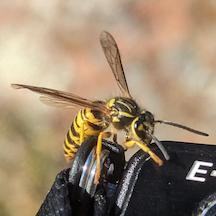
\includegraphics[width=\textwidth]{slide_img/wasp6.jpeg}
         \end{subfigure} 
         
        \begin{subfigure}[b]{0.2\textwidth}
             \centering
             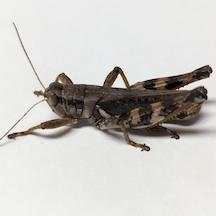
\includegraphics[width=\textwidth]{slide_img/grasshopper3.jpeg}
         \end{subfigure}   
         %
        \begin{subfigure}[b]{0.2\textwidth}
             \centering
             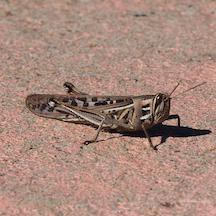
\includegraphics[width=\textwidth]{slide_img/grasshopper4.jpeg}
         \end{subfigure}
         %
        \begin{subfigure}[b]{0.2\textwidth}
             \centering
             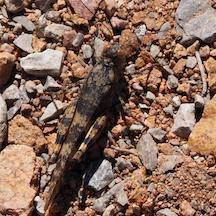
\includegraphics[width=\textwidth]{slide_img/grasshopper5.jpeg}
         \end{subfigure}
         %
        \begin{subfigure}[b]{0.2\textwidth}
             \centering
             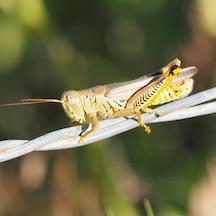
\includegraphics[width=\textwidth]{slide_img/grasshopper6.jpeg}
         \end{subfigure}
        
        \end{center}
        \caption{Dataset 1: wasps vs grasshoppers (more diverse)}
    \end{figure}


    \begin{figure}
        \begin{center}
        \begin{subfigure}[b]{0.2\textwidth}
             \centering
             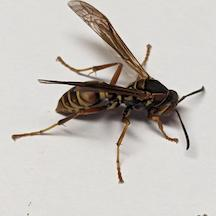
\includegraphics[width=\textwidth]{slide_img/wasp4.jpeg}
         \end{subfigure}   
         %
        \begin{subfigure}[b]{0.2\textwidth}
             \centering
             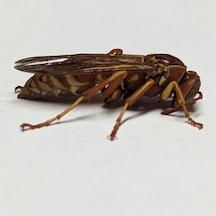
\includegraphics[width=\textwidth]{slide_img/wasp5.jpeg}
         \end{subfigure}
         %
        \begin{subfigure}[b]{0.2\textwidth}
             \centering
             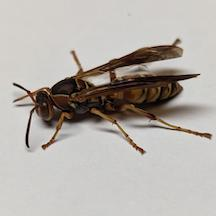
\includegraphics[width=\textwidth]{slide_img/wasp3.jpeg}
         \end{subfigure}
         %
        \begin{subfigure}[b]{0.2\textwidth}
             \centering
             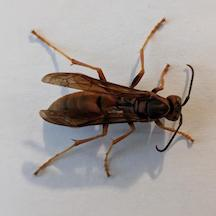
\includegraphics[width=\textwidth]{slide_img/wasp7.jpeg}
         \end{subfigure}
         
        \begin{subfigure}[b]{0.2\textwidth}
             \centering
             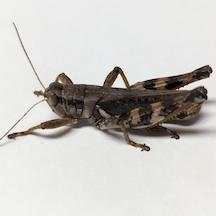
\includegraphics[width=\textwidth]{slide_img/grasshopper3.jpeg}
         \end{subfigure}   
         %
        \begin{subfigure}[b]{0.2\textwidth}
             \centering
             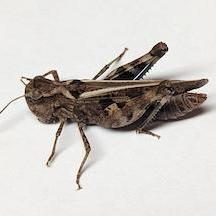
\includegraphics[width=\textwidth]{slide_img/grasshopper2.jpeg}
         \end{subfigure}
         %
        \begin{subfigure}[b]{0.2\textwidth}
             \centering
             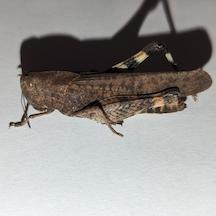
\includegraphics[width=\textwidth]{slide_img/grasshopper1.jpeg}
         \end{subfigure}
         %
        \begin{subfigure}[b]{0.2\textwidth}
             \centering
             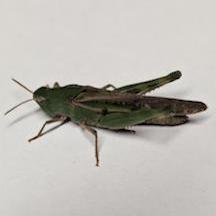
\includegraphics[width=\textwidth]{slide_img/grasshopper7.jpeg}
         \end{subfigure}
        
        \end{center}
        \caption{Dataset 2: wasps vs grasshoppers (less diverse)}
    \end{figure}
}
\end{minipage}

\end{frame}

\subsection{Diversity Framework}
\begin{frame}
\frametitle{Diversity Framework}

\begin{minipage}[t]{0.35\textwidth}
    \only<1-4>{\begin{figure}
        \centering
        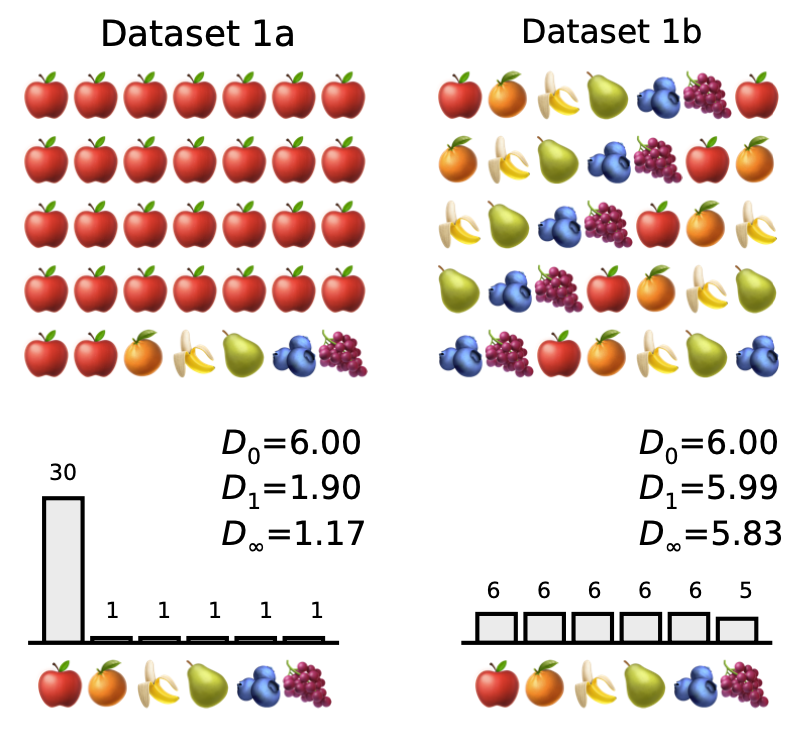
\includegraphics[width=0.9\textwidth]{slide_img/fruits-1.png}
        \caption{Diversity depends on frequency, image taken from \cite{greylock}}
    \end{figure}}

    
    \only<5->{\begin{figure}
        \centering
        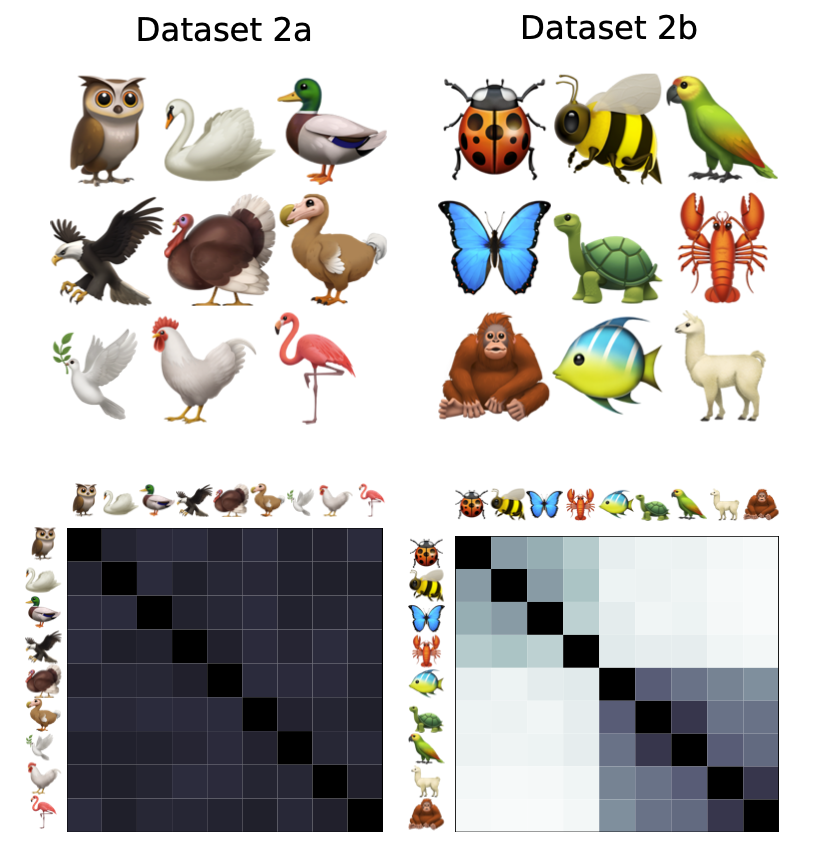
\includegraphics[width=0.9\textwidth]{slide_img/similarity.png}
        \caption{Diversity depends on similarity, , image taken from \cite{greylock}}
    \end{figure}}
\end{minipage}
%
\begin{minipage}[t]{0.55\textwidth}
    \begin{itemize}
        \item \onslide<1->{How do we measure \textbf{diversity}?}
        \begin{itemize}
            \item \onslide<2->{We will use the framework of Leinster and Cobbold \cite{leinster2012} and Reeve et al. \cite{reeve2016}}
            \item \onslide<3->{This framework generalizes the Hill numbers \cite{hill1973}}
            \item \onslide<4->{Like Hill numbers, this framework accounts for the frequency with which different types of things occur}
            \item \onslide<5->{Unlike Hill numbers, it also accounts for the similarities between types. Higher similarities lead to lower diversities}
        \end{itemize}
        \item \onslide<6->{In the context of an image classification training set \ldots}
        \begin{itemize}
            \item \onslide<7->{We will consider each image to be a unique type}
            \item \onslide<8->{The similarity between images will be based on their euclidean distance in pixel space (smaller distance $\leftrightarrow$ higher similarity)}
        \end{itemize}
        \item \onslide<9->{We can also treat class balance in this framework by using a similarity matrix based on sharing the same class label}
    \end{itemize}
\end{minipage}
    
\end{frame}

\section{Methodology}
%\begin{frame}
%\sectionpage
%\end{frame}

\begin{frame}
\frametitle{Methodology}

\begin{minipage}[t]{0.55\textwidth}
\begin{enumerate}
    \item \onslide<2->{Collect a number datasets}
    \begin{itemize}
        \item \onslide<3->{PathMNIST, BloodMNIST, OrganAMNIST, and OrganCMNIST from MedMNIST \cite{medmnistv1, medmnistv2}}
        \item \onslide<4->{Several additional datasets, including those used in Madani et al. \cite{madani2018} and Chinn et al. \cite{Chinn2021}}
    \end{itemize}
    \item \onslide<5->{From each dataset, sample the training set to create many subsets}
    \item \onslide<6->{Train a neural network classifier on each subset, and measure the performance of this classifier against a test set (common to subsets from the same parent dataset)}
    \item \onslide<7->{Measure an assortment of diversity indices for each subset (including class balance)}
    \item \onslide<8->{Use linear regression to measure how much variation in model performance is explained by different sets of diversity indices.}
\end{enumerate}
    
\end{minipage}
%
\begin{minipage}[t]{0.35\textwidth}

\begin{figure}
    \centering
    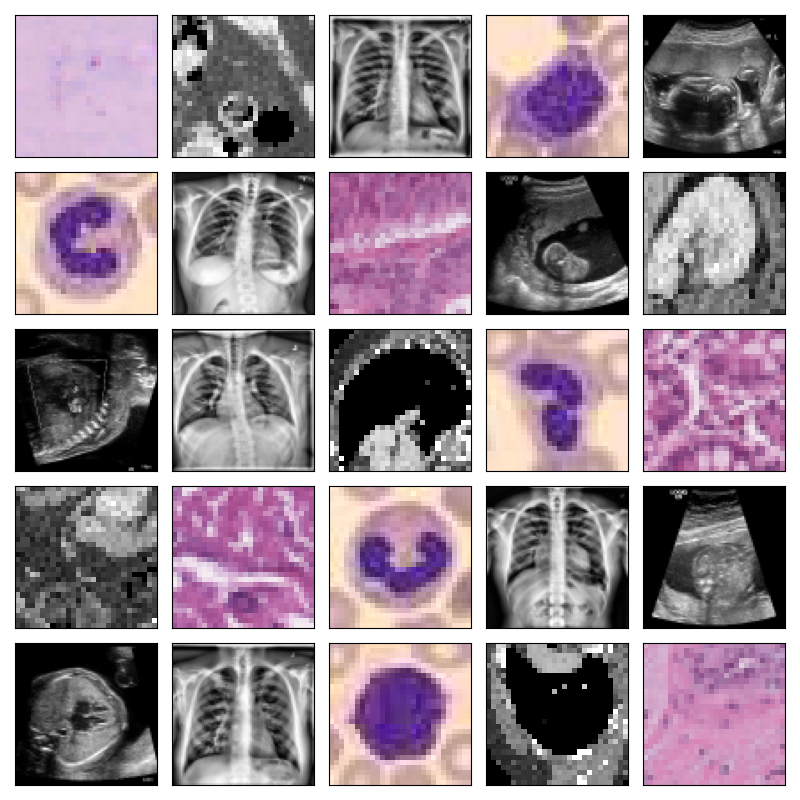
\includegraphics[width=0.9\textwidth]{slide_img/image_grid.png}
    \caption{Images from some of the selected datasets}
\end{figure}

\end{minipage}
    
\end{frame}

\section{Preliminary Results}
%\begin{frame}
%\sectionpage
%\end{frame}

\begin{frame}
\frametitle{Preliminary Results}

\begin{minipage}[t]{0.4\textwidth}

    \only<1-5>{\begin{figure}
        \begin{center}
            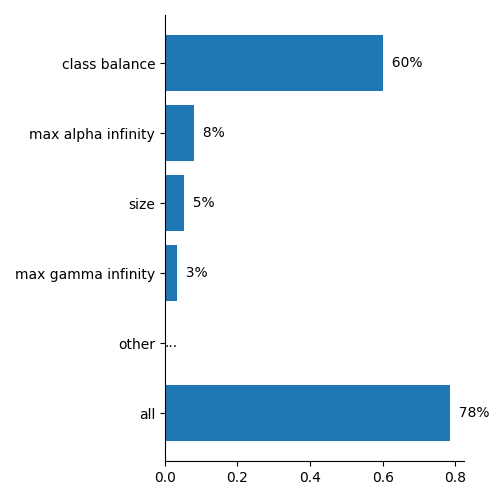
\includegraphics[width=\textwidth]{slide_img/R_squared_by_feature_cum_barh.png}   
        \end{center}
        \caption{Additional variance of performance explained by feature}
    \end{figure}}
    
    \only<6>{\begin{figure}
        \begin{center}
            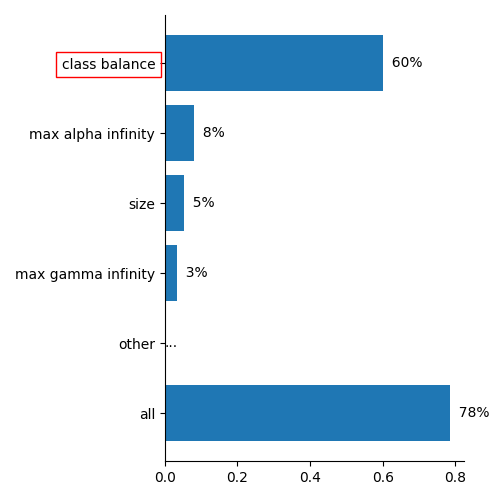
\includegraphics[width=\textwidth]{slide_img/R_squared_by_feature_cum_barh2.png}   
        \end{center}
        \caption{Additional variance of performance explained by feature}
    \end{figure}}
    
    \only<7>{\begin{figure}
        \begin{center}
            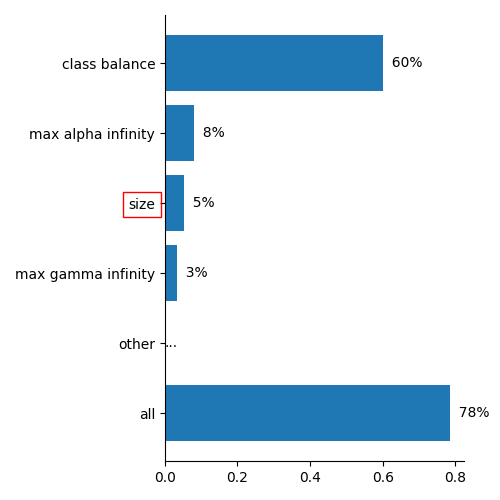
\includegraphics[width=\textwidth]{slide_img/R_squared_by_feature_cum_barh3.png}   
        \end{center}
        \caption{Additional variance of performance explained by feature}
    \end{figure}}
    
    \only<8>{\begin{figure}
        \begin{center}
            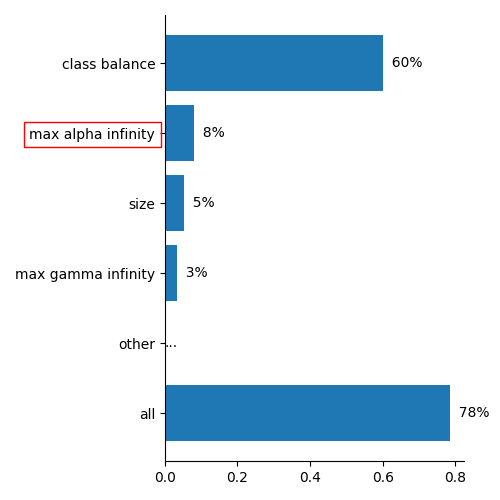
\includegraphics[width=\textwidth]{slide_img/R_squared_by_feature_cum_barh4.png}   
        \end{center}
        \caption{Additional variance of performance explained by feature}
    \end{figure}}
    
    \only<9>{\begin{figure}
        \begin{center}
            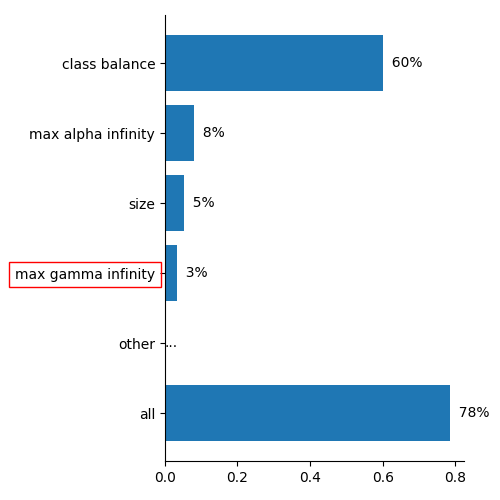
\includegraphics[width=\textwidth]{slide_img/R_squared_by_feature_cum_barh5.png}   
        \end{center}
        \caption{Additional variance of performance explained by feature}
    \end{figure}}
    
    \only<10->{\begin{figure}
        \begin{center}
            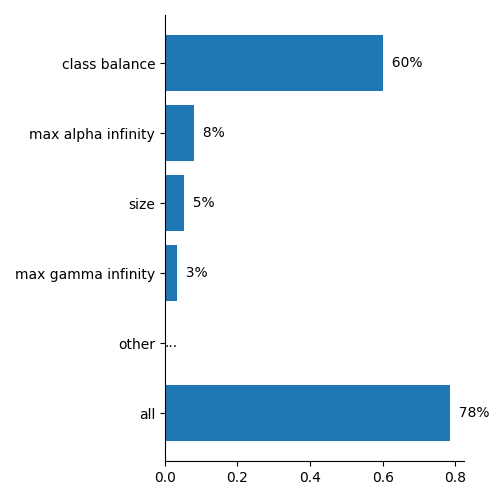
\includegraphics[width=\textwidth]{slide_img/R_squared_by_feature_cum_barh.png}   
        \end{center}
        \caption{Additional variance of performance explained by feature}
    \end{figure}}
\end{minipage}
%
\hfill
%    
\begin{minipage}[t]{0.55\textwidth}

    \begin{itemize}
        \item \onslide<2->{Using only class balance and size, we achieve an $R^2$ of approximately $68\%$ }
        \begin{itemize}
            \item \onslide<3->{I.e., these two features jointly explain about 2/3 of the variance across all datasets in the performance of models trained on those datasets.}
        \end{itemize}
        \item \onslide<4->{$\leftarrow$ Here we have the $R^2$ by feature} 
        \begin{itemize}
            \item \onslide<5->{These features were found using a greedy search. Reported $R^2$ contribution is the difference in $R^2$ before and after that features is included.}
            \item \onslide<6->{Class balance is the most important ($R^2 \approx 0.60$)}
            \item \onslide<7->{Subset size becomes the third most important}
            \item \onslide<8->{A different diversity measure from the diversity framework turns out to be more important than subset size}
            \item \onslide<9->{A second diversity measures from the diversity framework turns out to be similarly important}
            \item \onslide<10->{The top four features explain about $77\%$ of the variance in performance}
            \item \onslide<11->{The remaining features add only an additional $\approx 1\%$}
        \end{itemize}
        \item \onslide<12->{In summary, we have quantified the importance of class balance, and demonstrated that other diversity indices contribute to dataset quality}
        \item \onslide<13->{\textbf{We are testing on multiple datasets, and would love to test on more. If you have data that might benefit from this approach, we would love to collaborate, just reach out!}}
    \end{itemize}

\end{minipage}
\end{frame}

\begin{frame}
\frametitle{Thank you for attending my talk!}

%\begin{center}

\vspace{0.02\textwidth}

Websites:
\begin{itemize}
    \item arnaoutlab.org
    \item arnaoutlab.ucsf.edu
\end{itemize}

\vspace{0.02\textwidth}

Contact Info:
\begin{itemize}
    \item JC: jcouch1@bidmc.harvard.edu
    \item Ramy Arnaout (PI): rarnaout@bidmc.harvard.edu
    \item Rima Arnaout (PI): rima.arnaout@ucsf.edu
\end{itemize}
    
%\end{center}
    
\end{frame}

\begin{frame}
\frametitle{References}
{\tiny
\bibliographystyle{JHEP} %JHEP.bst
\footnotesize\bibliography{main}
}
\end{frame}

\end{document}
